\section{Track reconstruction with pixel detectors}\label{sec:Tracking with pixel}
%\pagestyle{plain}
Precise tracking is a fundamental tool for any collider experiment. An efficient identification of electrons and muons, based on tracking, is a key factor for a correct reconstruction of the final states of collisions events.\\
It is important to determine the position of the interaction point, the primary vertex, moreover some particles do not decay promptly after the production and they neither live enough to transverse the full detector, i.e. hadrons containing b and c-quarks and the $\tau$-lepton.
%Hadrons composed of a b or c quark and a lighter quarks (as $D^0$ and $B^0$), have a lifetime dominated by the decay of the heavier quark, which is mediated via the weak interaction. The life-time at rest of these particles is of the order of magnitude of the \SI{}{\pico\second}.
%The $\tau$-lepton has a rather large mass compared to the other two charged leptons and a lifetime $\tau_{rest} = \SI{290}{\femto\second}$\cite{tau_life}.
All these particles have in common that they decay inside or close to the innermost detector layer, but on average live long enough to have their decay detected by measuring the position of their decay vertex, the secondary vertex.\\
% Particles produced in high-energy experiment are usually highly relativistic. Since the life-time of a boosted particle is  $\tau_{boosted} =\gamma \tau_{rest}$, the secondary vertex will be displaced from the primary vertex, the secondary vertex can be then measured and identified, i.e. a $\tau$-lepton of \SI{100}{\GeV} momentum extend travels for $\sim$\SI{5}{\milli\meter} in average.\\
Pixel detectors play a fundamental role in tracking and vertex identification thanks to their high density of readout channel, good time resolution and the high radiation hardness.
The high density of channel lead to a high spatial resolution, this feature is extremely important for being able to distinguish each of the tracks in dense environment, so that pixel detectors can be used for pattern recognition purposes.
The high rate of collision of LHC requires also detectors to be very fast, and operate at the typical \SI{40}{\mega\hertz} rate. Pixel detectors meet this requirement thanks to fast transistors with dimension of the order of \SI{200}{\nano\meter}. This detection technique is ideal for operating close to the IP due to its radiation hardness performance.
%The radiation hardness performance of silicon devices, used both as front-end readout and detective bulk, makes pixel detector ideal candidates for operating close to the IP of particle physics experiment.
%Their tracks are superimposed on those produced in the rare high-\pt collisions leading to very complex patterns that can be reconstructed efficiently only by high granularity devices with good time resolution.
%At the \TeV-scale the pattern recognition has the additional challenge of precisely reconstructing the tracks of narrow jets produced by highly boosted low mass particles like highly energetic b-jets.\\
In this chapter the mechanism of charged particles detection, tracking in magnetic field and vertices discrimination will be covered.
\subsection{Particle interaction with matter}
A particle could interact with the material that is crossing through either losing some of its own energy or deflecting its trajectory. Those property are used to detect particle flow in the particle detectors.
The energy loss could happen either via electromagnetic or nuclear interactions, involving the atom's electrons and nuclei.
Particles detectors are mainly distinguished by the mechanism they use to reveal the particles and the type of particles they are devoted to detect, i.e. tracking detectors normally detects charged particles via ionization interaction.
In this section a brief description of the main interaction processes in tracking detectors will be presented.
%Particles interact with matter through several processes that depends on the characteristichs of the particles themselves and of the material that they cross.


\subsubsection{Interaction of charged particles}
The description of the energy loss of a charged particle through ionization phenomena is provided by the Bethe-Block formula\cite{bethe_block}, a quantum-mechanical correction to the Bohr formula which uses a classical electro-dynamic approach.
The mean energy loss per lenght $<\frac{dE}{dx}>$ is:
\begin{equation}
-<\frac{dE}{dx}>~=~\frac{4\pi r^2_e m_ec^2 N_A Zz^2 \rho}{A\beta^2}\bigg( \frac{1}{2} ln\bigg( \frac{2m_e c^2 \beta^2 \gamma^2 T_{max}}{I^2}-\beta^2 -\frac{\delta(\beta \gamma)}{2} \bigg) - \frac{C}{Z}  \bigg)
\end{equation}
where $Z$ and $A$ are the atomic and the mass number of the material, $\rho$ is the material density, $N_A$ is the Avogadro constant and $r_e=\SI{2.8}{\femto\meter}$ is the classical electron radius, $z$ is the charge of the incident particle in unity of electrons, $\beta = \frac{v}{c}$ and $\gamma = \frac{1}{\sqrt{1-\beta^2}}$, where $c$ is the speed of light. The mean excitation energy of the material $I\simeq I_0Z$ with $I_0 \simeq 12 \eV$ when $Z<13$. $T_{max}$ is the maximum kinetic energy which can be imparted to a free electron in a single collision. C is the shell correction.
The density correction $\delta$ is an effect which becomes important at high energy, the incident particle is polarizing the material while crossing it. This produces a shield effect on atoms far from the particle, reducing the energy loss.
\begin{figure}
\center
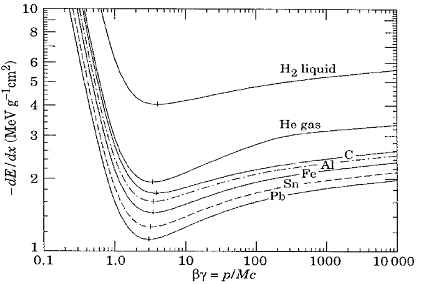
\includegraphics[width=0.6\textwidth]{./Images/tracking_det/BetheBlock.png}
\caption{The Bethe-Bloch equation solved for numerous materials in case of a single charge particle.}
\label{pic:bethe}
\end{figure}
As a function of $\beta \gamma$ the energy loss has no dependency on the mass of the incident particle. The Bethe-Block formula is valid in the $\beta \gamma$ range from 0.05 and 500, outside this range other processes than ionization are dominant.\\
Figure \ref{pic:bethe} shows the mean energy loss of a particle crossing a material as a function of its $\beta \gamma$.
Due to the small increase above the minimum, all the particles with $\beta \gamma~>~3$ are commonly called Minimum Ionizing Particles. This condition is typical of the collision products of the LHC.
The calculation of energy loss depends on the width of the absorber media. For thick absorber the distribution of energy loss is gaussian, given the high number of interactions. For thin absorber the number of interaction is low and the energy loss distribution is not gaussian. A theoretical calculation was provided by Landau\cite{landau}, Symon and Vavilov based on the parameter $\kappa = \frac{\overline{\Delta}}{W_{max}}$, where $\overline{\Delta}$ is mean energy transferred in a single scattering and $W_{max}$ is the maximum energy that can be trasferred in a single scattering process.
The Landau theory is valid for $\kappa \le 0.01$ and it assumes that $W_{max}\rightarrow \infty$, the trasferred energy is high enough that the electrons could be considered as free, the speed of the incident particle remains constant in the scattering process. The integral transport equation can be solved under these hypothesis.
\begin{equation}
\frac{df}{dx}(x,\Delta) = \int_0^{\infty}W(E)[f(x,\Delta - E)-f(x,\Delta)]\mathrm{d}E
\end{equation}
Here $f(x,\Delta)$ represents the distribution probability that the incident particle will lose an amount $\Delta$ of energy on traversing a layer of thickness x. $W(E)dE$ denotes the probability per unit path length of a collision transferring energy E to an electron in the material. The function $W(E)dE$ is not generally known, an approximate solution by using the free electron (Rutherford) cross section that matches with the hypothesis:
\begin{equation}
W(E) = \frac{\xi}{x} \frac{1}{E^2} \quad \& \quad \frac{\xi}{x}=0.1535\frac{z^2 Z \rho}{A \beta^2 } 
\end{equation}
The Landau distribution is therefore given by:
\begin{equation}
\begin{split}
f_L(x,\Delta) = \frac{\phi(\lambda)}{\xi}\quad \& \quad \phi(\lambda) = \frac{1}{\pi} \int_0^{\infty}e^{ -t \mathrm{ln}(t) -\lambda t  } sin(\pi t) \mathrm{d}t 
\\
\lambda = \frac{\Delta -\overline(\Delta)}{\overline{\Delta}} -\mathrm{ln}(\frac{\overline{\Delta} 2mc^2 \beta^2}{(1-\beta^2)I^2})- 1 +C_E
\end{split}
\end{equation}
where $C_E=0.5772$ is the Eulero constant.
The Landau distribution, $f_L(x,\Delta)$, is asymmetric with a tail extending to $E_{max}$. This tail is mainly due to fast emitted $\delta$-rays, electrons with enough energy to escape a significant distance away from the primary radiation beam and produce further ionization. The energy loss corresponding to the maximum of the function $f_L(x,\Delta)$ is the most probable energy loss.
\begin{figure}
\center
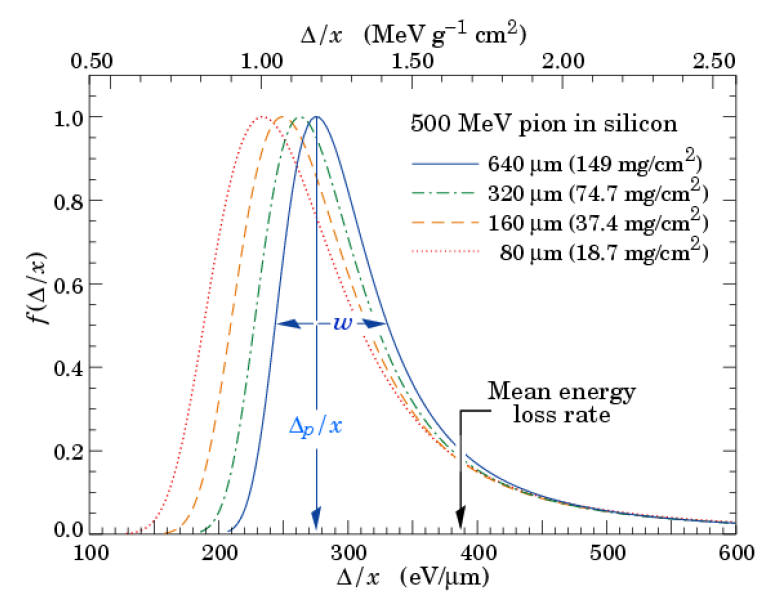
\includegraphics[width=0.6\textwidth,height=0.45\textwidth]{Images/tracking_det/Landau.jpg}
\caption{Landau functions in silicon for 500~MeV pions, normalized to unity at the most probable value $\Delta_p/x$. The Landau distribution is shown for different widths of silicon layers.}
\label{pic:landau}
\end{figure}
Figure \ref{pic:landau} shows the typical Landau distribution for different widths of silicon layers for an incoming 500~\MeV pion.
%dSeveral mechanisms describe the energy loss of a particle into the material: ionization of the atoms of the material, emission of Cherenkov radiation, emission of transition radiation, bremmsstrahlung processes and nuclear reactions. The first three are electromagnetic processesand they are dominant for particles with low momentum.
\subsubsection{Particle scattering}
In addition to inelastic collisions with the atomic electrons, particles passing through matter undergo repeated elastic Coulomb scattering from nuclei although with a smaller probability.
Considering that usually nuclei have mass greater than the incoming particle, the energy transfer is negligible but each scattering centre adds a small deviation to the incoming particle's trajectory also. Even if this deflection is small, the sum of all the contribution adds a random component to the particles path which proceed with a zig-zag path. As result, particles show a deviation from the incoming trajectory after having crossed a material.
Three possibility can be considered:
\begin{itemize}
\item Single scattering. When the thickness is extremely small and the probability to have more than one interaction is negligible. In this case the situation is well described by Rutherford formula\cite{rutherford}: 
\begin{equation}
\frac{d\sigma}{d\Omega} = \big(\frac{1}{4\pi\epsilon_0} \big) \frac{ z_1^2 z_2^2 e^4}{M^2c^4\beta^4} \frac{1}{sin^4(\frac{\theta}{2})}
\end{equation}
\item	Plural scattering. When the number of Coulomb scattering increases but remains under few tens of interactions. This is the most difficult case to deal with, several works have been done by different authors\cite{plural_scattering}.
\item Multiple scattering\cite{multiple_scattering}. When the thickness increases and the number of interactions become high the angular dispersion can be modeled as Gaussian.
\end{itemize}
Multiple scattering is the most common situation. The angular dispersion can be calculated as:
\begin{equation}
\sigma_{\Theta_0} = \frac{13.6 MeV}{\beta c p}z \sqrt{\frac{x}{X_0}}[1+0.038\mathrm{ln}(\frac{x}{X_0})]
\label{eq:mult_scat}
\end{equation}
where p is the momentum, z is the charge of the incident particle and $\frac{x}{X_0}$ is path in radiation length in the absorber material.
% The standard deviation $\sigma_0$ of this distribution depdends on the radiation lenght $X_0$ of the material, the momentum $p$, a
Multiple scattering contributes to the uncertainty on the track reconstruction. Reducing the detector thickness and using material with larger $X_0$ decrease the standard deviation of the scattering angle distribution.
\subsubsection{Interaction of neutral particles}
Charged particles are not the only one contributing to energy release in the matters, also release of energy from neutral radiation needs to be considered.
Significant contributions come from photons and from neutral hadrons as neutrons. The two type of particles interact in a very different way and have different impact on tracking performance.
Photons can interact in many ways with the material via electromagnetic interactions. The type of interaction depends on the atomic number of the material Z and of the energy of the photons themselves.
\begin{figure}
\center
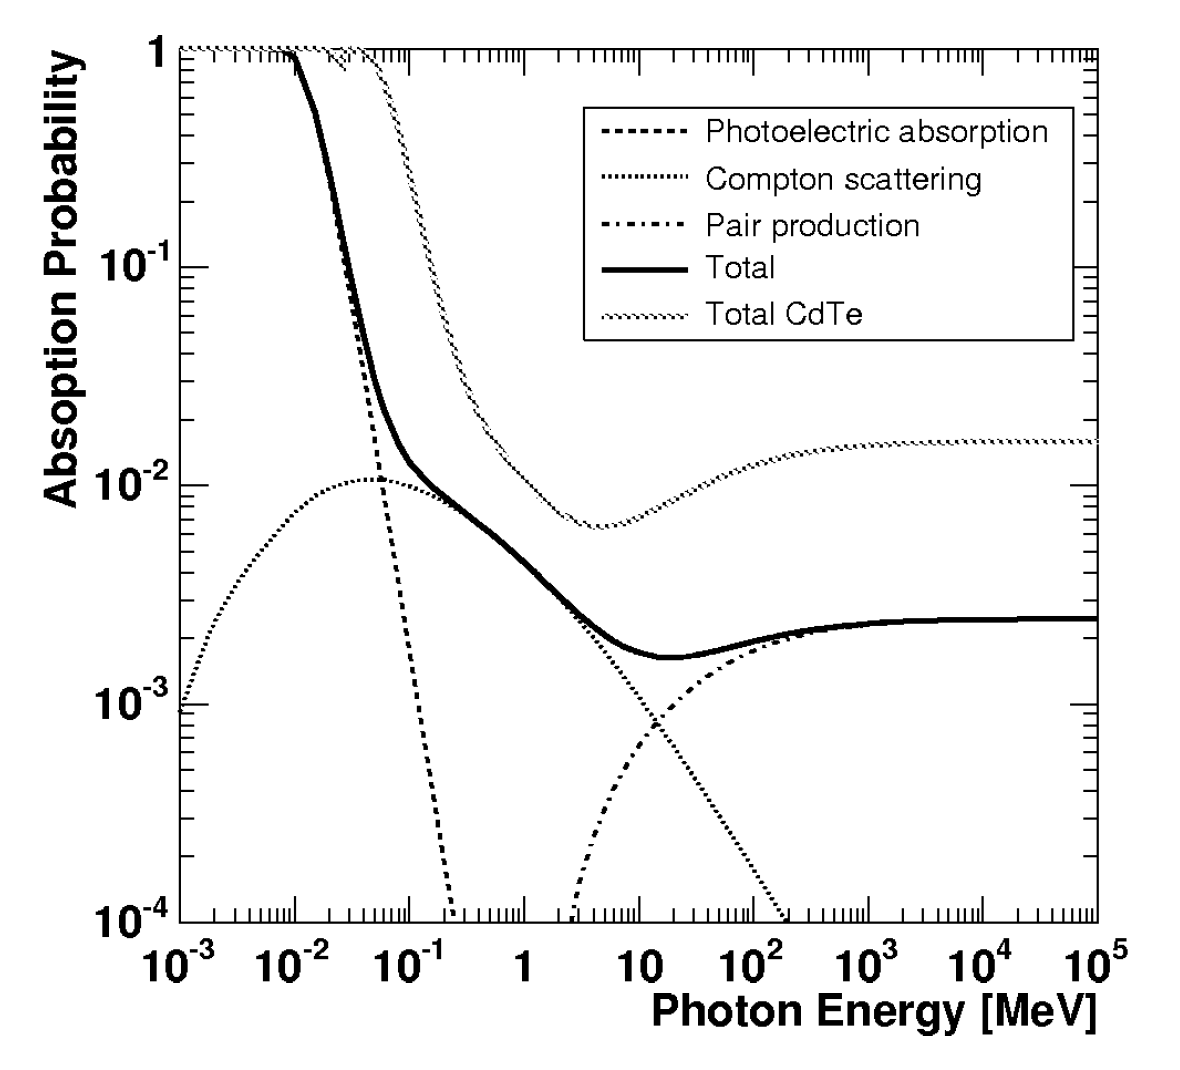
\includegraphics[width=0.5\textwidth]{Images/tracking_det/photon_interaction.png}
\caption{Mass attenuation coefficient of the silicon and its components.}
\label{pic:photon_interaction}
\end{figure}
Figure \ref{pic:photon_interaction} shows the mass attenuation coefficient of photons in silicon and the contribution from different processes. Mass attenuation coefficient characterizes how easily a material can be penetrated by a beam and it is defined as $\frac{\mu_a + \mu_s}{\rho}$, where $\mu_a$ is the absorption coefficient, $\mu_s$ is the scattering coefficient and $\rho$ the material density. Several types of photon interaction with matter are possible, the most probable are:
\begin{itemize}
\item Photoelectric effect: which is the most probable interaction for energy lower than \SI{0.1}{\MeV}
\item Compton effect: which is the most probable interaction in the energy range \SIrange{0.1}{100}{\MeV}
\item Pair production via bremsstrahlung: which is the most probable interaction for energy higher than \SI{100}{\MeV}
\end{itemize}
%While photoelectric absorption and Compton effect are dominant at low photon energy ($E_{\gamma}<\SI{100}{\MeV}$), at high energy the dominant process is the pair production via bremsstrahlung. 
In the LHC environment photons are typically high energetic and the pair production mechanism is the dominant one and it will be taken in consideration in the following text.
Although pair production is the key-process for photon identification in the calorimetry, it is a background phenomenon that could lead to fake reconstructed tracks and vertices in the Inner Detector.
In this process the photon interacts with an electron or a nucleus producing a positron-electron pair. In order to produce the pair the photon must have at least an energy of 1.022\MeV. In Figure~\ref{pic:photon_interaction} the two components of the pair production cross section are shown, respectively for the interaction with nuclei or electrons.\\
Neutron can interact with matter by strong interaction with nuclei. In general strong interaction could happen also with charged hadrons, as protons, but it is rare with respect to electromagnetic interaction, though, with the high fluences of LHC it needs to be well monitored and described because of the radiation damage that will cause.
For a strong interaction to happen the hadron needs to be at $\simeq$~\SI{10}{fm} from the nucleus. The type of neutron interaction will depend upon the energy of the neutron and the mass number of the material itself, here a list of the most important phenomena:
\begin{itemize}
\item Elastic scattering, which is dominant in the MeV region;
\item Inelastic scattering, in which the nucleus is excited and then decays with the production of $\gamma$. This phenomenon has a energy threshold of about 1~\MeV;
\item Neutron capture, corresponding to the process $n+(Z,A)\rightarrow \gamma + (Z,A+1)$, which is dominant for low energy neutrons (\eV-\keV);
\item Other nuclear reactions, which typically happen for low energy neutrons (\eV -\keV);
\item Production of hadronic showers, for very high energy neutrons ($\simeq$~100~\MeV)
\end{itemize}
The cross section of neutron interaction is proportional to the velocity of the neutron itself, as $1/v_n$, this means that the most interacting neutrons are the low energetic ones, which are then the most dangerous one for devices that needs to operate in a radioactive environment. Details about the radiation damage will be treated later in this thesis work.
% Another possible interaction, but usually negligible compared to the previous ones is the Photonuclear reaction, in this case the photon interact directly with the nucleus. The related cross section is shown in Figure 1 in dotted line (σg.d.r.). 
%A suitable quantity, often used to characterize the absorption of a photon shower, is the mass attenuation coefficient. The mass attenuation coefficient is defined as:
%\begin{equation}
%\mu_m = \eta_A \frac{\sigma_{tot}}{\rho}
%\end{equation} 
%where 

\subsection{Properties of pixel silicon detector}
\begin{figure}
\centering
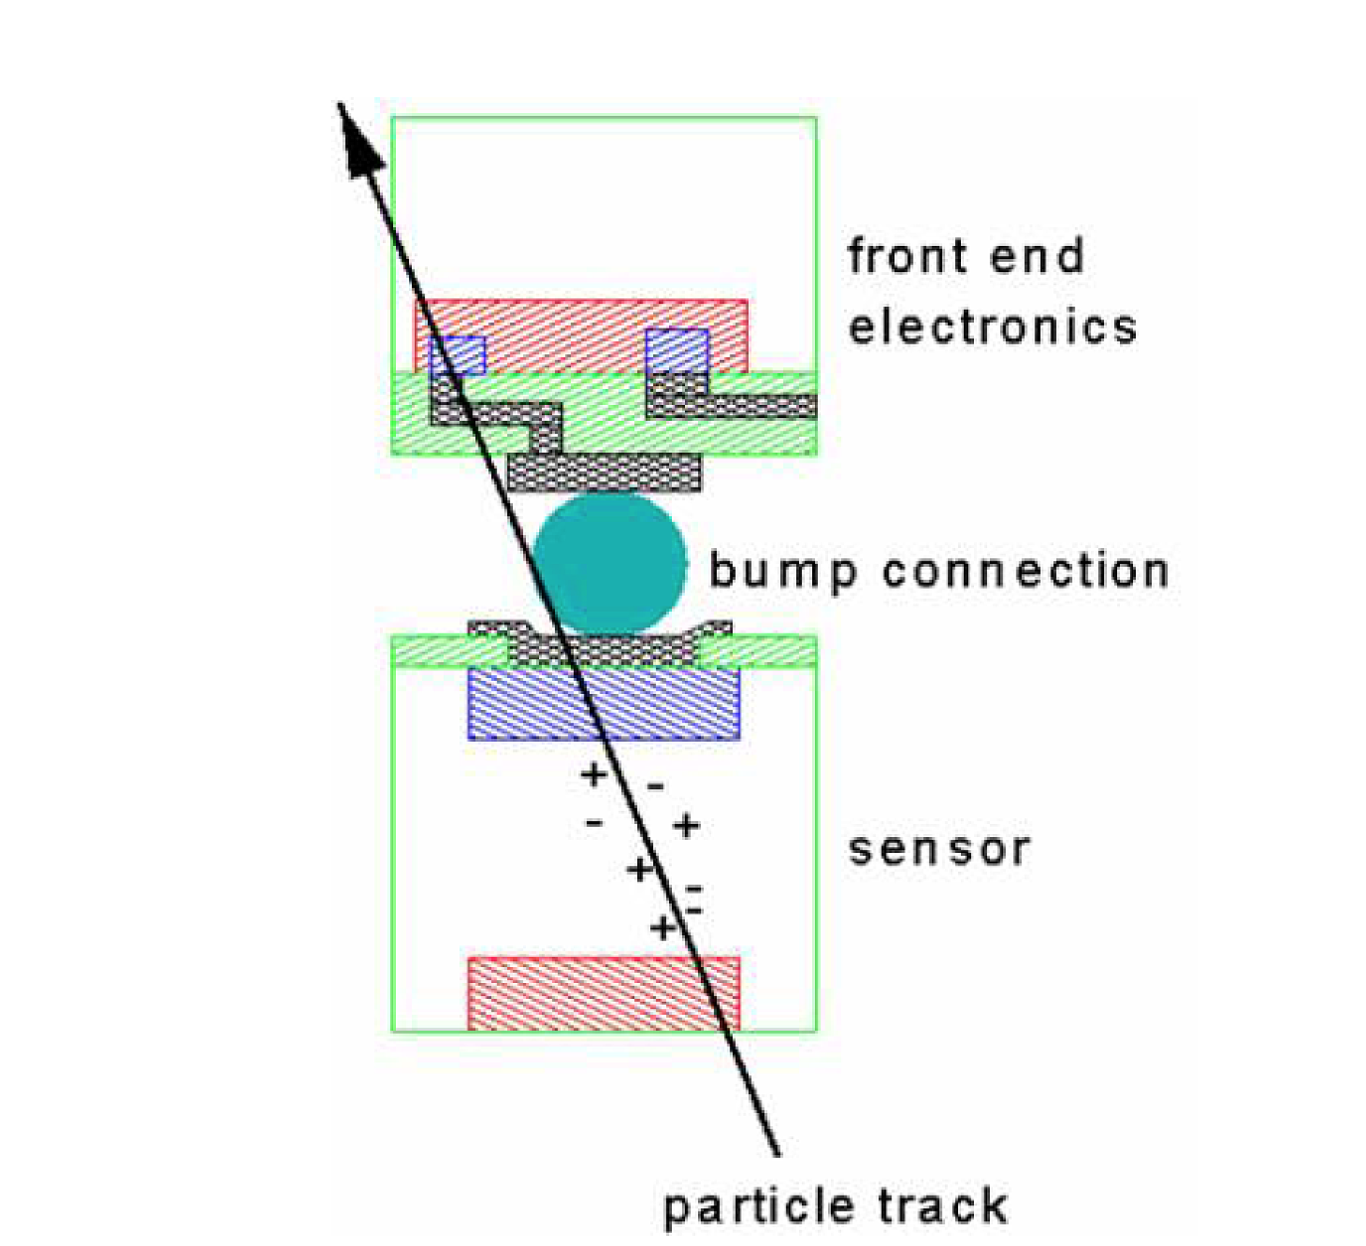
\includegraphics[width=0.4\textwidth]{Images/tracking_det/hybrid.png}
\caption{Cross section of hybrid pixel readout channel. Sensor, at the bottom, provides the signal generation, the bump, in the middle, provides the interconnection and the readout chip, at the top, takes care of the signal amplification and the data processing.}
\end{figure}

The main tasks of the pixel detector is the pattern recognition and the measurement of momentum for charged tracks. Additionally pixel detectors contribute to the resolution of the secondary vertices from the primary vertex. Pixel detectors are made of silicon sensors. The choice of silicon as a bulk material is motivated by the radiation hardness performance, the possibility to achieve a fine segmentation, the good time resolution and the high availability which drives the relatively low cost.
A brief description of the main properties and the most important aspects that need to be consider in silicon detectors follows.\\
There are two possible option for pixel silicon sensors, either the readout electronics is integrated on the sensor itself (monolithic sensor) or the readout electronic is integrated in an external chip, connected to each pixel of the sensor (hybrid sensor). Radiation hard design of the silicon sensor typically requires the use of high voltage bias, so that a radiation hard monolithic sensors is possible only if the electronics is well protected from the bias applied to the bulk, as it is possible using the HVCMOS technology. The use of HVCMOS technology is currently investigation and it was not considered for the construction of the ATLAS pixel silicon sensors, whose approach was the use of hybrid sensors.\\
The working principle of hybrid sensors is shown in Figure~\ref{fig:hybrid}, the signal is created in the silicon sensor and then transmitted to the readout chip connected to the sensor via a metallic bump.

\subsubsection{Signal generation in silicon sensors}

%An ionizing particle crossing a silicon layer transfers energy to the silicon atoms. In the band theory \cite{band-theory} this is described by the creation of electron-hole pairs, which can move through the silicon. Although the width of the forbidden gap of silicon is only 1.1 \eV, in average 3.6 \eV are needed to create an electron-hole pair in silicon since the lattice excitation also absorb energy. Silicon detectors use this mechanism to generate a signal whenever a charged particle is crossing their volume.\\

Silicon is a semiconductor, this means that electrons that are bounded to the silicon atoms can be freed and let the silicon being conductive if a relatively small amount of energy it is transferred to them. This principle is well described in the band theory \cite{band-theory} with the concept of energy gap, which is the minimum energy that an electron required in a material to move freely in the structure. In silicon the energy gap is $\sim$\SI{1.1}{\eV}, this mean in average \SI{3.6}{\eV} are needed to free an electron from a silicon atom, because most of the energy is lost within the lattice structure. The electron is then free to move around the silicon lattice and it contributes to the electrical conductivity of the material.\\
The lack of an electron in the crystal bounds is as well participating to the electrical conductivity, in the lattice electrons from other atoms could fill the vacancy, and those electrons will be affected by any external field applied to the silicon, taking part to the electrical conductivity. This phenomenon could be schematized thinking the vacancy of an electron in the silicon crystal acting as a positive charge, also called hole. The electrical conductivity can  be then describe in term of electrons, referring to the contribution of free electrons inside the lattice, and holes, referring to the contribution of bounded electrons of the lattice.\\
As previously said, when a ionizing particle crosses a material, it transfer energy to the material by ionization effect.
In semiconductors this energy is high enough to let an electron leave the atom and so to create and electron-hole pair. The same happen in metals, but without an energy threshold, so that thermal effect dominates and the creation of the signal cannot be discriminate.\\
\begin{figure}
\center
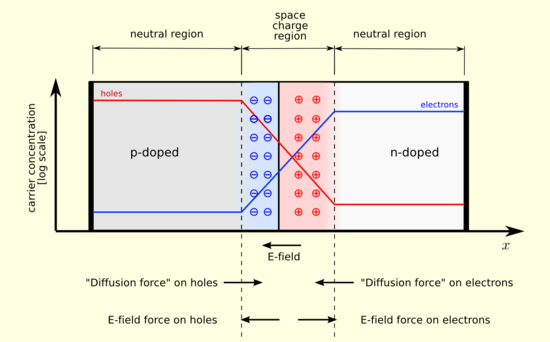
\includegraphics[width=0.6\textwidth]{Images/tracking_det/pn-junction.png}
\caption{Schematic view of a p-n junction}
\label{pic:pn-junction}
\end{figure}
Another property that makes silicon a good material for particle detection is the possibility of doping it to modify its electrical properties. Doping is a process in which impurities are diffused in the silicon, with local modification of the lattice structure. Doping can be p-type, where borum atoms replace some of the silicon atoms in the lattice structure, or n-type where phosphorus atoms are use instead. In the p-type silicon, given the 3 valency electrons of the borum instead of the 4 of the silicon, one of the bound of the borum with the surrounding silicon atoms is made by a single electron, instead of a couple. The net effect of p-type borum is to increase the number of holes in the lattice structure. In the n-type silicon, phosphorus atoms have 5 valency electrons, 4 of them are used to create bounds with the surrounding silicon atoms and one is free to move in the crystal.\\
Doping is widely used in electronics to create p-n junction non-linear devices as diodes and transistors. A diode is a p-n junction, a device in which the silicon is doped with two different doping. In a p-n junction the two different types of doping are made next one to each other in a silicon crystal. Since the two doped materials have different concentrations of electrons and holes, free electrons from n-type side will diffuse in the p-type region and free holes of p-type will go in the n-type one. This process will create a region depleted by free charge and in which there is a built-in electrical field due to the charge of the ions (borum and phosphorus), the depletion region, as shown in Figure~\ref{pic:pn-junction}.\\
Silicon sensors are simple diodes where the collecting electrodes, made of heavily doped silicon (typically the concentration of doping centers is higher than \SI{e15}{\per{\cubic{\centi\meter}}}), are implanted on a poorly doped bulk (doping concentration in the range \SIrange{e12}{e14}{\per{\cubic{\centi\meter}}}). Two type of electrodes are present in a silicon detectors, one with an opposite-type doping with respect to the bulk and another with same-type doping but higher concentration. The first forms the p-n junction with respect to the bulk, while the second is used as ohmic contact. Metal is not used to create an ohmic contact with the bulk because of the higher fermi level \cite{metal_semiconductor_juction}, which would effect in an additional current source in the device.\\
The depletion region is crucial in silicon detectors. When an ionizing particle is passing through the depletion region it generates holes and electrons which drift towards the electrodes because of the electric field, so that the possibility of recombination of the electron-hole pair is drastically reduced.
The depletion region can be enhanced applying a reverse bias to the diode, up to the entire volume of the sensor. The maximum voltage that one can impose while keeping the current across the diode low is called breakdown voltage. Silicon sensors are typically operated below the breakdown voltage, in order to limit the leakage current.\\
The speed of electrons and holes is directly proportional to the electric field;
\begin{equation}
\vv{v}_{h,e} = \mu_{h,e}(\abs{\vv{E}}) \vv{E}
\end{equation}
where $\mu_{h,e}$ is the mobility and it depends on material impurities and temperature.
\begin{figure}
\center
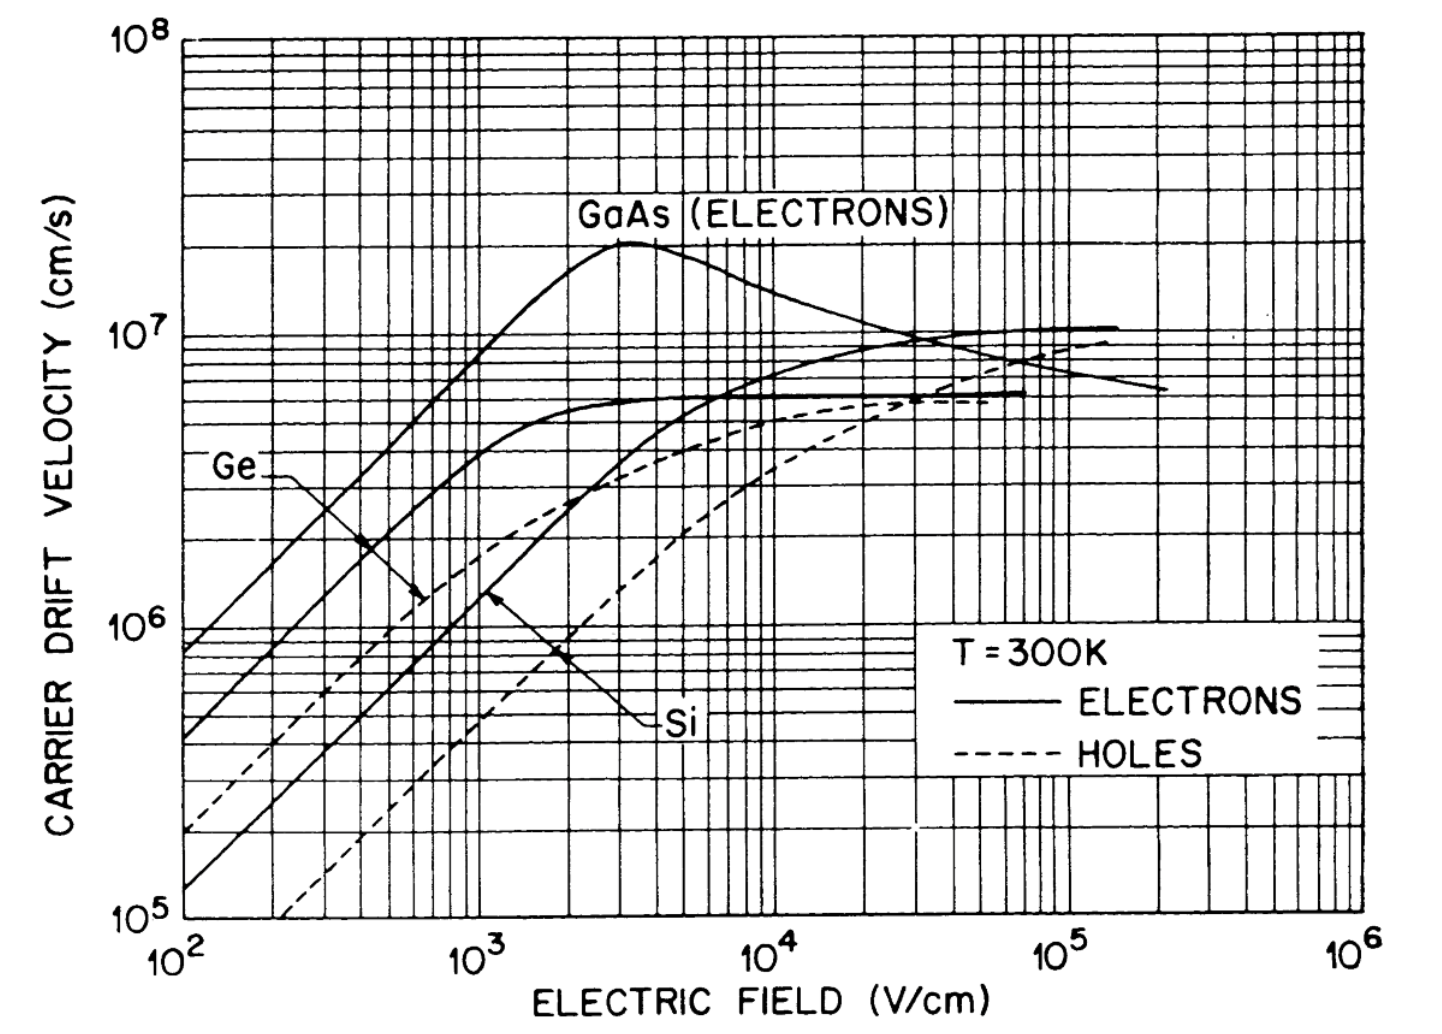
\includegraphics[width=0.6\textwidth]{Images/tracking_det/mobility.png}
\caption{Drift velocity as function of the electric field for different material at room temperature.}
\label{pic:mobility}
\end{figure}
Figure \ref{pic:mobility} shows the drift velocity as function of the applied electric field for silicon devices at room temperature.
Drift is not the only component to the holes and electrons movement in the silicon, thermal diffusion is acting as well as predicted from diffusion theory. The diffusion mechanism let the cloud of electron-hole pairs generated to spread with a gaussian trend around the generation point. The standard deviation of this gaussian is:
\begin{equation}
\sigma_{h,e} = \sqrt{2D_{h,e}t_{h,e}}
\end{equation}
where $D_{h,e}$ is the diffusion coefficient and $t_{h,e}$ is the lifetime for holes and electrons. Holes and electrons turn out to have roughly the same $\sigma$, because $D_{h,e}\propto \mu_{h,e}$ and $t_{h,e}\propto 1/\mu_{h,e}$, typical values are $\sigma \simeq \SI{10}{\micro\meter}$.
Given the Bethe-Block equation a single charge minimum ionizing particle is releasing \SI{1.66}{\MeV \square{\centi\meter}\per{\gram}} in silicon, which means that for a \SI{200}{\micro\meter} thick device $~14000$ electron-hole pairs are generated. Those numbers are very important to choose the proper threshold in the electronics.
The signal seen by the electrodes is an inducted signal, the movement of each single electron is contributing to the current at the electrode even when the charge are far from it. The typical signal duration depends on the applied voltage, the resistivity of the silicon and the thickness of device. Typically this is of the order of $\sim$\SI{10}{\nano\second}.

\subsubsection{Amplification and digitization of the signal}
The signal coming from the silicon sensor needs to be amplified and digitized for being transmitted to the data-acquisition system. These operations are performed at the level of the read-out chip, which is typically divided in a analog circuitry, responsible for the amplification and the digitization, and a digital circuitry, responsible for the delivering of the signal to the data-acquisition system.\\
The analog part of the circuitry faces directly the silicon sensors and it can use several techniques for the conversion of the signal in an amplified and square one. In the following the details about a charge sensitive amplifier will be given, since this is the strategy used for the read-out chip considered in this work of thesis.\\
\begin{figure}
\centering
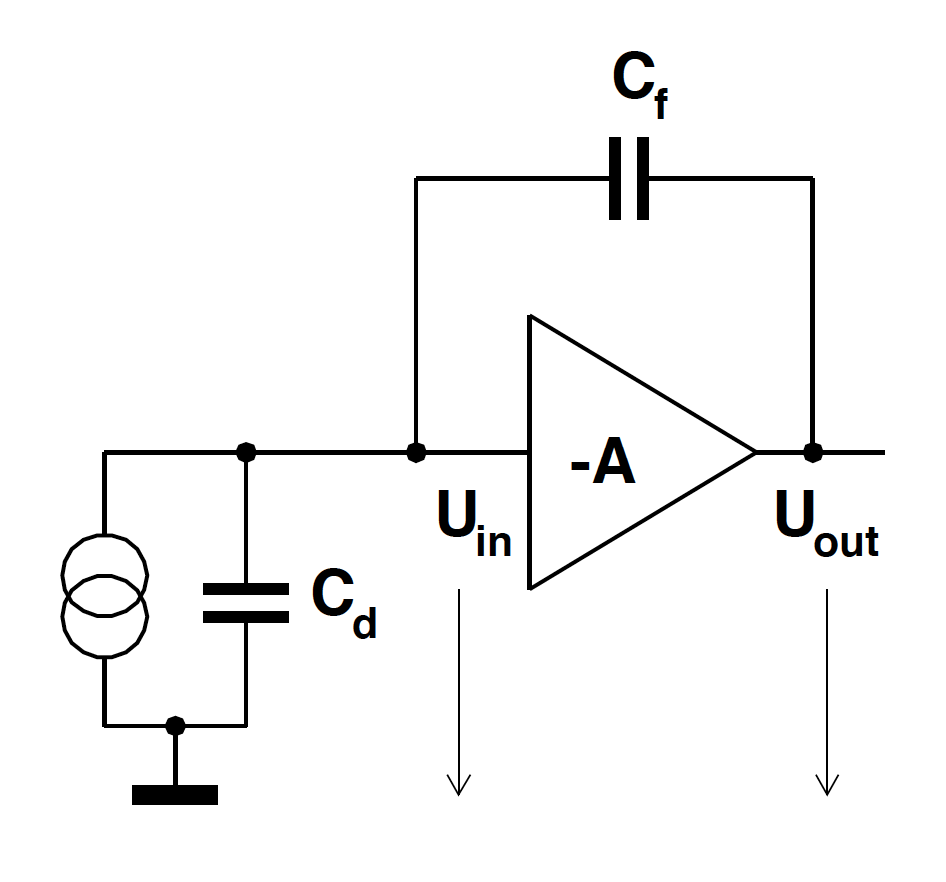
\includegraphics[width=0.5\textwidth]{Images/tracking_det/ChargeSensitiveAmplifier.png}
\caption{Principle of a charge-sensitive amplifier}
\label{pic:amp}
\end{figure}
The principle of a Charge Sensitive Amplifier is shown in Figure~\ref{pic:amp}. The silicon sensor can be schematized as a current source in parallel with a capacitor, describing the capacitance of the sensor pad. The induced charge from the silicon sensor results in a voltage ($U_{in}$) at the amplifier input which is amplified to $U_{out}=-A U_{in}$. Ideally no current flows at the amplifier input and then the charge $Q_f$ on the feed-back capacitor $C_f$ and the charge $Q_d$ remaining on the detector capacity must add to the signal charge $Q_{coll}$. The voltage on $C_f$ is the difference between input and output voltage and thus:
\begin{equation}
Q_{coll} = Q_f + Q_d = U_out \cdot( C_f\frac{A+1}{A}-C_d\frac{1}{A})
\end{equation}
which yields the output voltage as function of induced charge:
\begin{equation}
U_{out} = \frac{Q_coll}{C_f\frac{A+1}{A}+\frac{C_d}{A}}\underrightarrow{A\rightarrow\infty}\frac{Q_{coll}}{C_f}
\end{equation}
so that the charge gain is easily controlled by only one parameter ($C_f$) in case of large amplification.
The feed-back capacitor of the Charge Sensitive Amplifier needs to be reset after a signal from the silicon sensor has been processed. This is achieved by either adding a resistor or a constant current source in parallel to $C_f$.
It is often desired to modify the shape of the signal pulse produced by the Charge Sensitive Amplifier, combining a low-pass and a high-pass filter to the amplifier, this is usually referred as shaper. The limiting frequency range that can pass the Charge Sensitive amplifier circuit is used to limit the bandwidth for noise to pass through the read-out circuit. Noise in electronic devices has three main origins:
\begin{itemize}
\item Thermal noise: caused by thermal fluctuations in the charge carrier distribution of any conductors; its power spectrum is constant in frequency and proportional to $k_BT$.
\item Shot noise: caused by fluctuations in the number of charge carriers when a boundary (e.g. a p-n junction) is crossed; its power spectrum is constant in frequency and proportional to the current crossing the boundary.
\item Low frequency noise: has a large variety of sources, e.g. charge trapping and release in semiconductors. The power spectrum is proportional to $f^{-\alpha}$, where $f$ is the noise frequency and $\alpha = 0.5 ... 2$.
\end{itemize}
A more detailed treatment of noise can be found in~\ref{Joern_25}.
The noise as seen after the analog part of the readout system is described by the variance of the output signal $<U_{out}^2>$ which is directly proportional to the noise power spectrum.
The noise contribution from the silicon sensor comes from shot noise of the leakage current $I_{leak}$, while the noise that comes from the amplifiers transistors corresponds to voltage fluctuations on the amplifier input, composed of low frequency and thermal noise.
The noise could be estimated as the charge needed on the read-out input in order to create an output signal on the sample amplitude as:
\begin{equation}
Q^2_{noise}=C^2_f \cdot <U^2_{out}> = c'_1(C_d +C_f)^2 \frac{1}{\tau} + c'_2 (C_d+C_f)^2 + c'_3I_{leak}\tau
\end{equation}
where $\tau$ is the time constant of the shaper.
In most of the vertex detectors the amount of information and channels is large enough to require the analog signal to be digitized already on the detector electronics, turning signal information into a digital bit-stream.
A discriminator is used to decide if a signal is sufficiently large to have been created by a particle hit, thus discarding a fraction of noise hits. The discriminator information ca be used to limit further processing to only those signals that have a hit reported (zero-suppression), thereby reducing the amount of data that has to be handled.\\
If the shape of the signal at the discriminator input is well controlled and the falling edge is significantly larger than the rise-time, the time that the signal remains above threshold (time-over-threshold, \tot) is related to the height of the signal and then proportional to the charge released in the silicon detector. The \tot is measured by detecting the rising and falling edges of the discriminator output and determining the time difference between both. In case of a linearly falling edge of the amplifier signal, the relation between signal height is approximately proportional to the measured \tot.
When a hit is to be measured by a discriminator, $time-walk$ may be of concern: due to a finite amplifier rise time, which is controlled by the amplifier supply current, the time at which the discriminator goes to logically on depends on the height of the signal itself, i.e. on the charge at the amplifier input. If the time-walk is too large, a hit with low charge might be detected too late and associated to a bunch-crossing later than the hit actually occurred. The setting of the amplifier supply current is therefore a compromise between power consumption and thus heat dissipation and the need to keep the time-walk as low as possible.

\subsubsection{Spatial resolution} 
The spatial resolution across a given direction is determined by the dimensions of the pixel, the charge sharing between neighboring pixels and the threshold of the readout electronics.
The minimum spatial resolution is obtained when a single pixel is collecting all the signal and so the charge is not shared among different pixels.
The resolution in this case can be calculated assuming a uniform particle occupancy across the pixel width and a full efficiency of detection. %Then the occupancy can be assumed to be constantly $l$ in the range $[-\frac{d}{2},\frac{d}{2}]$, where d is the detector segmentation across the direction considered.
The error on the position measurement is thus the standard deviation $\sigma$ of the distribution probability, which is:
\begin{equation}
\sigma = \sqrt{\frac{\int x^2 f(x) \mathrm{d}x}{\int f(x) \mathrm{d}x}} = \sqrt{\frac{\int_{-\frac{d}{2}}^{\frac{d}{2}} x^2 \mathrm{d}x}{\int_{-\frac{d}{2}}^{\frac{d}{2}}  \mathrm{d}x}} = \frac{d}{\sqrt{12}}
\end{equation}
where d is the pixel size across the considered direction.
\begin{figure}
\centering
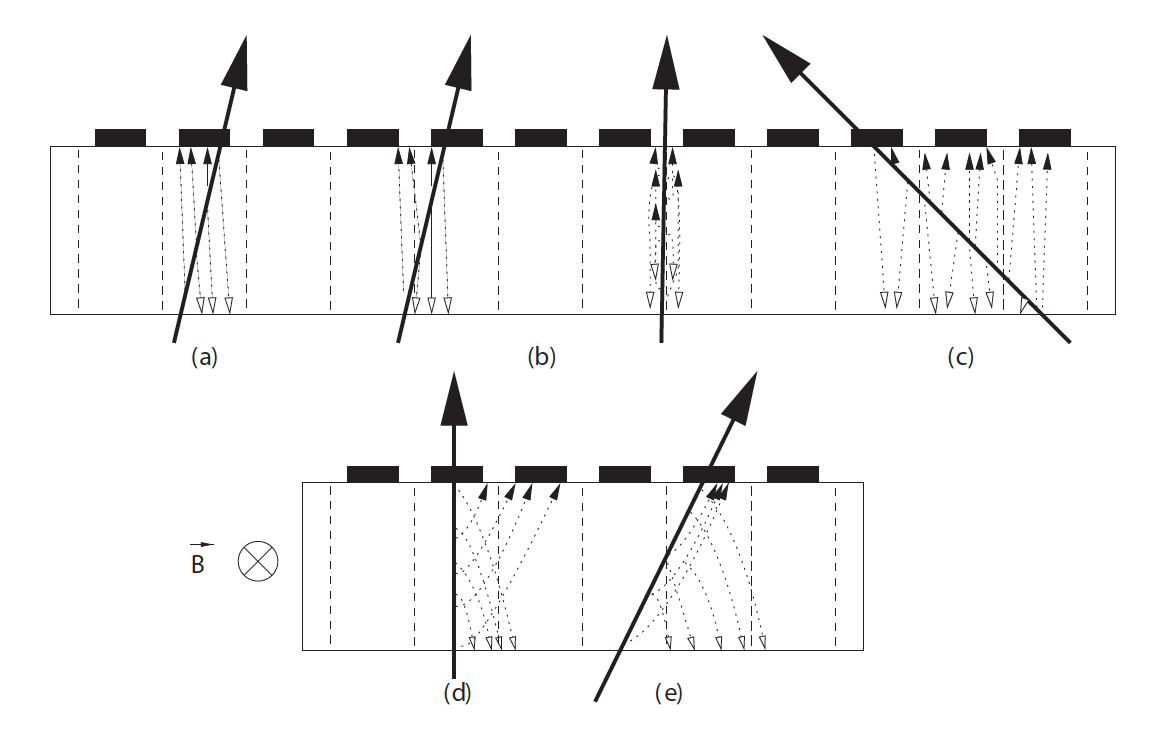
\includegraphics[width=0.8\textwidth]{Images/tracking_det/Lorentz.png}
\caption{The formation of clusters in a silicon detector~\ref{Joern_27}. The different types of arrows denote the polarity of the charge carriers while the big arrow indicates the particle tracks. Clusters are determined by the position and angle of the track. The presence of a magnetic shift leads to a Lorentz shift.}
\label{pic:Lorentz}
\end{figure}

When a particle cross the detector there is the possibility that more then one pixel could detect it. The different possibilities are shown in Figure~\ref{pic:Lorentz}. In particular a particle could pass in between the pixels (Figure~\ref{pic:Lorentz}(b)) or crossing the silicon detector with an angle so that releases charge in several pixels (Figure~\ref{pic:Lorentz}(c)). Another effect is the spread of the electron-holes cloud, but this contribution is limited by the strong electric field applied to the silicon sensors and typically the spread is in the order of few \SI{}{\micro\meter}, small if compared with the pixel size.
In case more then one pixel fires at the passage of a particle the informations provided by each of them are treated together in a single object, called cluster. The cluster is defined by its size, which is the number of pixel participating to it, its position, which is the center of charges of all the pixel, and its charge. %Commonly, center of gravity or eta calculations are used for this task.
%One possibility is diffusion which occurs during the entire drift of the charge carriers, which, for a silicon detector \SI{300}{\micro\meter} thick spreads the electron-holes cloud of a $\sigma_{max}\sim$\SI{4}{\micro\meter} and thus the charge sharing due to diffusion is limited to a region usually small compared to the pitch of the segmentation.
When the cluster size is greater than one, the resolution improves, because the position of the particle can be determined by the calculation of the centre of gravity of the charge. The reconstruction of the cluster is performed with neural network algorithms.
%Particles traversing the material under an inclination relative to normal incidence may have the released charge detected by several electrodes. The latter is due to the fact that an ionizing particle releases electron and holes across its entire path.\\
In case only an electric field is applied to separate the charge carriers, they drift along the direction of this field. If an additional magnetic field is present, as is the case in most tracking detectors, the path of the charge carriers deviates off the direction of the electric field due to the additional Lorenz force acting on the charges (Figure~\ref{pic:Lorentz}(d)). The effective angle of this deviation, the Lorentz angle $\theta_L$, is~\cite{Joern_27}:
\begin{equation}
tan\theta_L=\mu_{Hall}B_{\bot}
\end{equation}
where $B_{\bot}$ is the magnetic field perpendicular to the drift direction and $\mu_{Hall}$ is the Hall mobility, which is closely related to the mobility previously discussed.
The effect of the magnetic field is illustrate in Figure~\ref{pic:Lorentz}(d). It leads to a systematic shift of the detected position since detecting elements neighboring the actually hit electrode may see signals. The Lorentz angle may partially be compensated by inclining the detector with respect to normal particle incidence, as indicated in Figure~\ref{pic:Lorentz}(e). For strong electric fields, the dependency of the mobility $\mu$ on the field strength becomes important, also changing the Lorentz angle. This is an issue for silicon detectors after irradiation due to the increased depletion voltage.
While charge sharing is in general beneficial for the precision of the reconstruction of the track position, it also reduces the signal seen on each electrode which may this be below detection thresholds of the read-out electronics. The design of a silicon detector, in particular the inclination of the silicon sensors with respect to the expected particle direction, is therefore a compromise: the position resolution by charge sharing must be optimized while maintaining an efficient detection of signals.


\subsubsection{Radiation damage in silicon bulk}
\label{sec:rad_dam}

Silicon detector devices suffer from radiation damage due to the particles produced in the collisions, an issue which is particularly relevant at LHC experiments due to the high doses delivered to the tracking systems.
Incident particle at LHC have a sufficient energy to remove a silicon atom from the lattice. These collisions are mediated by Coulomb interaction in case of charged particles and by nuclear forces in case of neutral particle, in particular neutrons. Silicon atoms that are removed and get a sufficient amount of kinetic energy can remove other atoms from the lattice, resulting in a cascade of interactions.
Radiation-induced lattice damage is classified into point and cluster defects. Typically defects in the lattice are unstable, an interstitial atom is mobile and can fill a vacancy in another position.\\
The defects are of importance to the detector properties because they can create additional energy levels in the gap between valence and conduction band. Levels in the middle of the gap act mainly as generation and recombination centers given the similar distance to either band and thus similar access probability for electrons and holes. In contrast, levels close to the valence or conduction band act as trapping centers, i.e. electrons or holes are captured from the respective bands and released with a delay.
The trapping modifies the effective doping since free charge carriers are removed from the material. In a similar direction acts the combination of donor or acceptor atoms with vacancies or interstitial into stable defects. This has an effect on the depletion zone and on the bias needed for the full depletion. For large radiation doses, the depletion voltage may change from \SI{100}{\volt} to \SI{1000}{\volt}.
The charge trapping has also a consequence for the signal that is measured; the trapped charge carriers are released with a delay of the order of \SI{}{\micro\second} which is too long for the released electron (or hole) to be detected in the data-taking time window. The net signal measured is therefore smaller than for unirradiated devices, reducing detector performance. The trapping is usually characterized by a trapping costant $\tau^+$. The observed charge signal from a minimum ionized particle is reduced by $\Delta Q$ due to trapping for an originally created amount of charge carriers Q according to~\cite{moll}.
\begin{equation}
\frac{\Delta Q}{Q}=\frac{1}{3}(\frac{t_e}{\tau^+_e}+\frac{t_h}{\tau^+_h})
\end{equation}
where $t_{e,h}$ are the time for electrons or holes to reach the electrodes, respectively. The inverse trapping time constant is proportional to the particle fluence $\Phi$:
\begin{equation}
\frac{1}{\tau^+(\Phi)}=\frac{1}{\tau^+(0)} +\gamma \Phi
\end{equation}
with $\tau^+(0)\sim 0.51\cdot 10^6s^{-1}$ for both electrons and holes. For low fluences, the proportionality constant $\gamma$ is approximately the same for electrons and holes ($\gamma \sim \SI{0.24}{\square{\centi\meter}\per\second}$), however electrons show a stronger increase of $\frac{1}{\tau^+}$ above fluences of $\sim\SI{e14}{\square{\centi\meter}\per\second}$ normalized to 1\MeV neutrons \cite{moll}.
The generation-recombination centers lead to a additionally free electrons-hole pairs, that lead to an increase of current $\Delta I_{vol} = \alpha \Phi V$, with $\alpha\sim8\cdot10^{-14}\text{A}\SI{}{\per{\centi\meter}}$ for silicon at a temperature of $20^{\circ}C$ \cite{moll}. Another phenomenon that occurs after high radiation fluence is the change of properties of the bulk material, that led to an increase of the full depletion voltage. The increase of the depletion voltage has as consequence, the increase of the operative voltage of the device, with the subsequent increase in power consumption and a significant heat load to the device.If the heat load is not carried away effectively, the exponential dependency of $I_{vol}$ on the temperature will lead to an avalanche effect between increase of temperature and leakage current, also known as thermal runaway. Therefore sufficient cooling must be provided, with low temperature also reducing $\alpha$ and thus the extend of the radiation damage.\\
 The radiation induced defects in the silicon crystal structure that cause these degradation effects are most often not stable and consequently lead to a change of the sensor properties within time. The mobility of defects in silicon or their transformation is usually accelerated exponentially with temperature, a process known as annealing \cite{nicola_10}. Two stages are generally identified in the annealing process. In the first stage, known as beneficial annealing, part of the negative space charge generated by the defects is neutralized. Following this stage, the reverse annealing takes place, during which additional negative space charge is created in the sensor bulk \cite{nicola_10}. \\
The behavior of a silicon detector with respect to irradiation depends on the bulk doping of the silicon. N-type bulk undergoes to a phenomenon known as type inversion, that leads the concentration of p-type defects to increase with radiation, so that, at some point, the number of p-type defects becomes larger than the n-type ones. The net effect is the migration of the p-n juntion from the $p^+$ electrodes to the $n^+$, which needs to be considered in the design.\\
%The optimization of performance of silicon detectors for high radiation environment is a field in which many progress have been obtained in the recent years. 
Three main field were investigated in order to reduce the contribution of leakage current and to keep high performance even after high radiation doses: the defect engineering of silicon, the device engineering and the study of new materials.\\
Defect engineering of silicon consists in the deliberate incorporation of impurities or defects into the silicon bulk to improve the radiation tolerance of detectors. This is usually done enriching the silicon with oxygen during the production of the silicon lattice.\\%, which usually happens in Czochralski and Float Zone process.\\
Device engineering consists in the optimization of the design of the device. Several concepts have been developed so far. As already introduced p-doping is the best choice for device that have to stand high radiation doses, this translates in n$^+$-in-p devices, where the junction electrodes are made of heavily doped n-type silicon and the bulk is p-type silicon. Another choice is n$^+$-in-n device, in which the bulk is of n-type; in this device the junction is initially located to the electrodes not connected to the front-end readout chip, while after irradiation migrate to the front-end side. This was the baseline choice for the ATLAS Pixel Detector.\\
Another example of device engineering regards the geometry of the electrodes, for example making columnar electrodes that penetrates the silicon bulk can lower the full depletion voltage and makes the charge collection faster. This is the working principle of the 3D technology, described in details in Chapter 3.\\

%Extensive data concerning the development of Vdep in FZ p-on-n sensors with irradiation and annealing can be found in literature. The most accepted parametrization, the so called Hamburg Model, can be found in [10]. Other phenomenological studies and parameterizations on Float Zone p-on-n diodes and ministrip sensor properties with irradiation and annealing have been proposed [11?15]. The study presented in [11], in particular, gives a first evaluation of annealing effects on the charge collection efficiency of irradiated diodes. A decrease in the cluster charge is observed in type-inverted sensors after long annealing times. The technical design reports of HEP experiments always account for the effects of annealing, with a strict planning of room-temperature maintenance periods of the irradiated silicon tracking and vertex detectors. The aim of this work is to study the performance of irradiated FZ p-readout, n-bulk strip sensors in terms of signal and noise charge after irradiation and during annealing and to assess the operational limits and related performance losses in a harsh radiation environment like the ones present at the different LHC experiments.
%Radiation effects mitigate with time after irradiation stops, this phenomenon is known as annealing and it consists of vacancy being filled with a silicon atom or by transformation of a defect to another, changing the properties of the defect itself. The progress of the annealing depends strongly on the temperature of the device. Given that the second effect can result in larger defects on the long term, the initial beneficial effect of reducing the volume current can turn into its opposite (reverse annealing).\\

\subsubsection{Radiation damage in electronic read-out}
The electronic read-out is subject to radiation damage as well as the silicon bulk. A brief description of radiation damage for MOSFET (metal-oxide-semiconductor field effect transistor) technology \cite{MOSFET} follows, since this was the employed technology used of the IBL project.
In MOSFET technology the conduction is based on the flow of majority carriers below the SiO$_2$-Si interface. This region does not extend deeply into the bulk and so the net effect of radiation damages coming from displacement of silicon atoms is negligible up to 10$^{15}$ particles/cm$^2$.\\
The main source of radiation damage is due to ionization, generated by charged particles and photons. When ionizing radiation goes through a MOSFET, electron-holes paris are generated. Those charge quickly disappear in the gate metal contact and in the substrate, which have poor resistivity. The silicon dioxide used beneath the gate contact behaves differently because it is an insulator. 
\begin{figure}
\centering
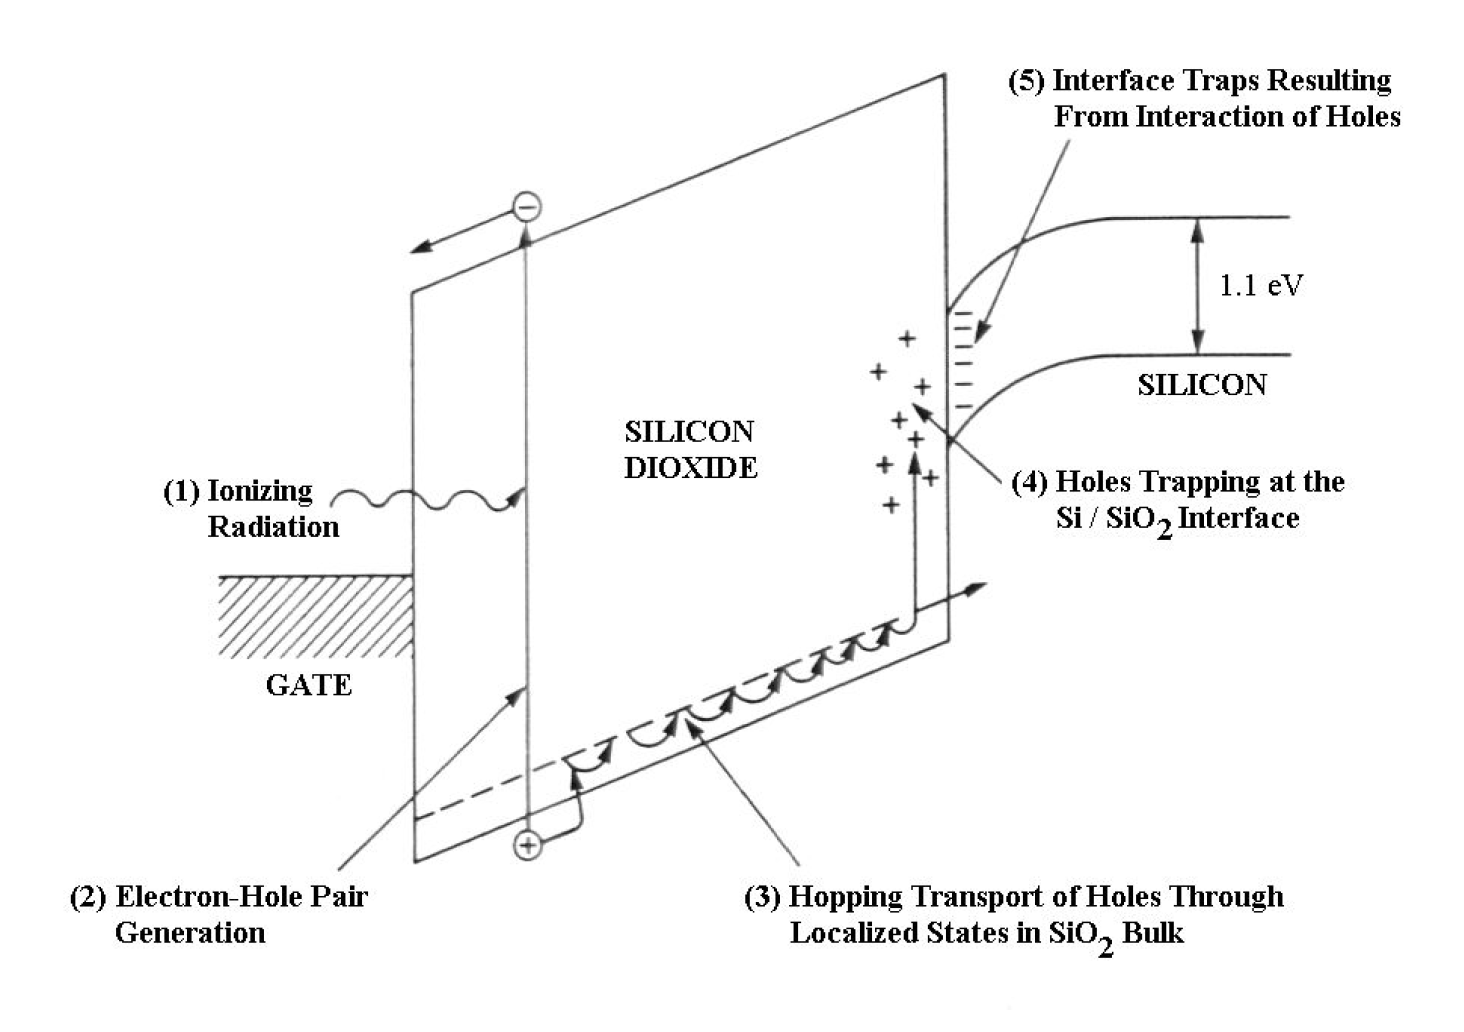
\includegraphics[width=0.8\textwidth]{Images/tracking_det/TID_damage.png}
\caption{Schematic illustration of the effects induced by ionizing radiation in a positively biased MOSFET device.}
\label{pic:MOSFET_rad_dam}
\end{figure}
Figure~\ref{pic:MOSFET_rad_dam} shows an illustration of the effect of ionizing radiation in a MOSFET device for positive gate bias. A fraction of the electron-hole pairs generated the ionizing particles will recombine each other, the rest of them will drift towards the gate because of its field. While the electrons will leave the oxide easily, hole can get trapped in the silicon defects due to the much smaller mobility, from five to twelve orders of magnitude lower. The latter phenomenon lead to a change of properties of the device with irradiation.\\
A first effect is the change of the threshold voltage of the device, which is the minimum gate-to-source voltage differential that is needed to create the conductive path between the source and the drain terminals. The oxide trapped charge gives origin to a threshold voltage shift proportional to the density of trapped holes and to the position of the charge distribution in the oxide with respect to the SiO$_2$-Si interface: the closer the charge to the 
SiO$_2$-Si interface is, the bigger the threshold voltage shifts. Hence, the threshold voltage of a NMOS\footnote{MOSFET obtained in n-type silicon bulk} transistor decreases because of the positive bias applied to the gate, whilst the one of a PMOS\footnote{MOSFET obtained in p-type silicon bulk} increases (in absolute value).\\
Another effect is the increase of leakage current after irradiation. Leakage current in a MOSFET is defined as the current which flows from drain to source when V$_{gs}$=\SI{0}{\volt} and V$_{ds}$=V$_{dd}$, and it is referred as
leakage current. Only NMOS transistors undergo an increase in the off-state current after irradiation. Two effects lead to this increase: the increase of the sub-threshold current and the generation of parasitic currents.\\
The decrease of the transistor threshold and the consequently increase of the leakage current are compensated by a counter-mechanism after few \SI{}{\mega\radian} of TID. At higher TID interface states start to appear in the silicon dioxide. The negative charge trapped in the interface states (in the case of NMOS transistors) only starts to compete with the oxide-trapped charge with some delay, giving origin to the rebound effect. From this point on the interface states contribute significantly to the charge balance at the transistor edge, increasing the threshold voltage of the parasitic lateral transistor and hence decreasing the leakage.\\
In addition to the changes of threshold voltage and leakage current, ionizing radiation affects other transistor parameters. The build-up of interface traps degrades the mobility of the carriers in the transistor channels. The trapping and releasing of the carriers increase the noise of the device.
The quantitative effects of the radiation on the device depends upon the its design. Radiation tolerance can be improved by several techniques as the reduction of the gate dimensions or using special layouts and architectures in the design phase. Transistors at LHC needs to stand a high level of TID, in particular for the innermost layer of the Pixel Detector the requirement is to stand \SI{300}{\mega\radian}.\\
Radiation can lead not only to permanent damages of the devices, but as well to transient effects that comes with a high linear energy transfer from charged heavy particles.  These particles, in particular ions created in hadronic interactions, can change the state of the transistor hitting the depleted gate region. This effect is called Single Event Upset (SEU) and it can lead to wrong information stored in or transmitted by the chip. A technique to correct for this effect is the replication of the memory cells combined with a majority vote logic.\\


\subsection{Tracking and tagging with the Inner Detector}
\subsubsection{Tracking in magnetic field}
The trajectory of a charged particle of momentum $p$ and charge $q$ in a static magnetic field is given by:
\begin{equation}
\frac{\mathrm{d^2}\vv{r}}{\mathrm{d}s^2} = \frac{q}{p} \frac{\mathrm{d}\vv{r}}{\mathrm{d}s}\times \vv{B}(\vv{r})
\end{equation}
where $\mathrm{d}s = v\mathrm{d}t$ is the distance along the trajectory. The vector $\frac{\mathrm{d^2}\vv{r}}{\mathrm{d}s^2}$ is perpendicular to the trajectory and its length is $1/R$, where $R(s)$ is the curvature radius of the trajectory; the vector $\frac{\mathrm{d}\vv{r}}{\mathrm{d}s}$ is tangent to trajectory and it has unit length. The integral
\begin{equation}
\int\mathrm{d}\alpha = \int \frac{\mathrm{d}s}{R} = \int \abs{\frac{\mathrm{d^2}\vv{r}}{\mathrm{d}s^2}} \mathrm{d}s = \frac{q}{p} \int \abs{\frac{\mathrm{d}\vv{r}}{\mathrm{d}s}\times \vv{B}(\vv{r})} \mathrm{d}s
\end{equation}
provides the bending angle of a charged particle in a magnetic field environment.
The transverse displacement $\delta$ of a particle after a path length $\ell$ perpendicular to the magnetic field is $\delta = \ell \alpha /2$, for $\ell <<R$.
%In high-energy physics experiments the coordinates are memeasured with position sensitive detectors.
The reconstructed cluster from the detectors are analyzed by a pattern recognition program that associates coordinates measurements to tracks.
At large momentum the trajectory can be approximated with a straight line $Y=a+bZ$ in the plane containing the magnetic field and with a parabola $Y=a+bX+(c/2)X^2$ in bending plane perpendicular to the magnetic field. The parameter of the quadratic term is related to the momentum of the particle in the bending plane $p_t$ through the radius of the circumference $c = -R^{-1}$.
The most popular approach to track finding is the combinatorial Kalman filter where the full knowledge of the tracks parameters at each detector layer is used to find compatible measurements in the next detector layer, forming combinatorial tree of track candidates.
A Kalman filter is usually applied to linear dynamic systems, which at every step k are described by a state vector $\vv{r}$. The evolution of the state vector from step $sk-1$ to step k is described by the linear transformation:
\begin{equation}
\vv{r}_k = F_{k-1}\cdot \vv{r}_{k-1} + \vv{w}_{k-1}
\end{equation}
where $F_{k-1}$ is the propagation matrix and $\vv{w}_{k-1}$ is a random noise contribution to the system during the propagation step. At every step a new measurement constrains the system, where the measurements $\vv{m}_k$ needs to be described as a linear function of the state vector $\vv{x}_k$ with associated Gaussian noise $\vv{\epsilon}_k$;
\begin{equation}
\vv{m}_k = H_k \vv{x}_k + \vv{\epsilon}_k
\end{equation}
Given such a linear dynamic system, the Kalman filter provides:
\begin{itemize}
\item Filtering: the optimal recursive estimator of the present state vector $\vv{x}$ given all previous measurements
\item Prediction: the optimal estimation of the state vector at a future time, given all past measurements.
\item Smoothing: an improved estimation of the state vector at some time in the past, given all measurements up to the present time.
\end{itemize}
In the case of track fitting, the various steps $k$ need to be interpreted as the various clusters to be added to a track along the track path: at each step $k$ the track helix is propagated to a new layer of the detector, through the propagation matrix F$_k$ and adding both the noise due to the multiple scattering and eventual energy losses due to radiation and the new measurement is added in linearized form, according to the linearization matrix H$_k$.



\subsubsection{Impact parameter resolution}
\begin{figure}
\center
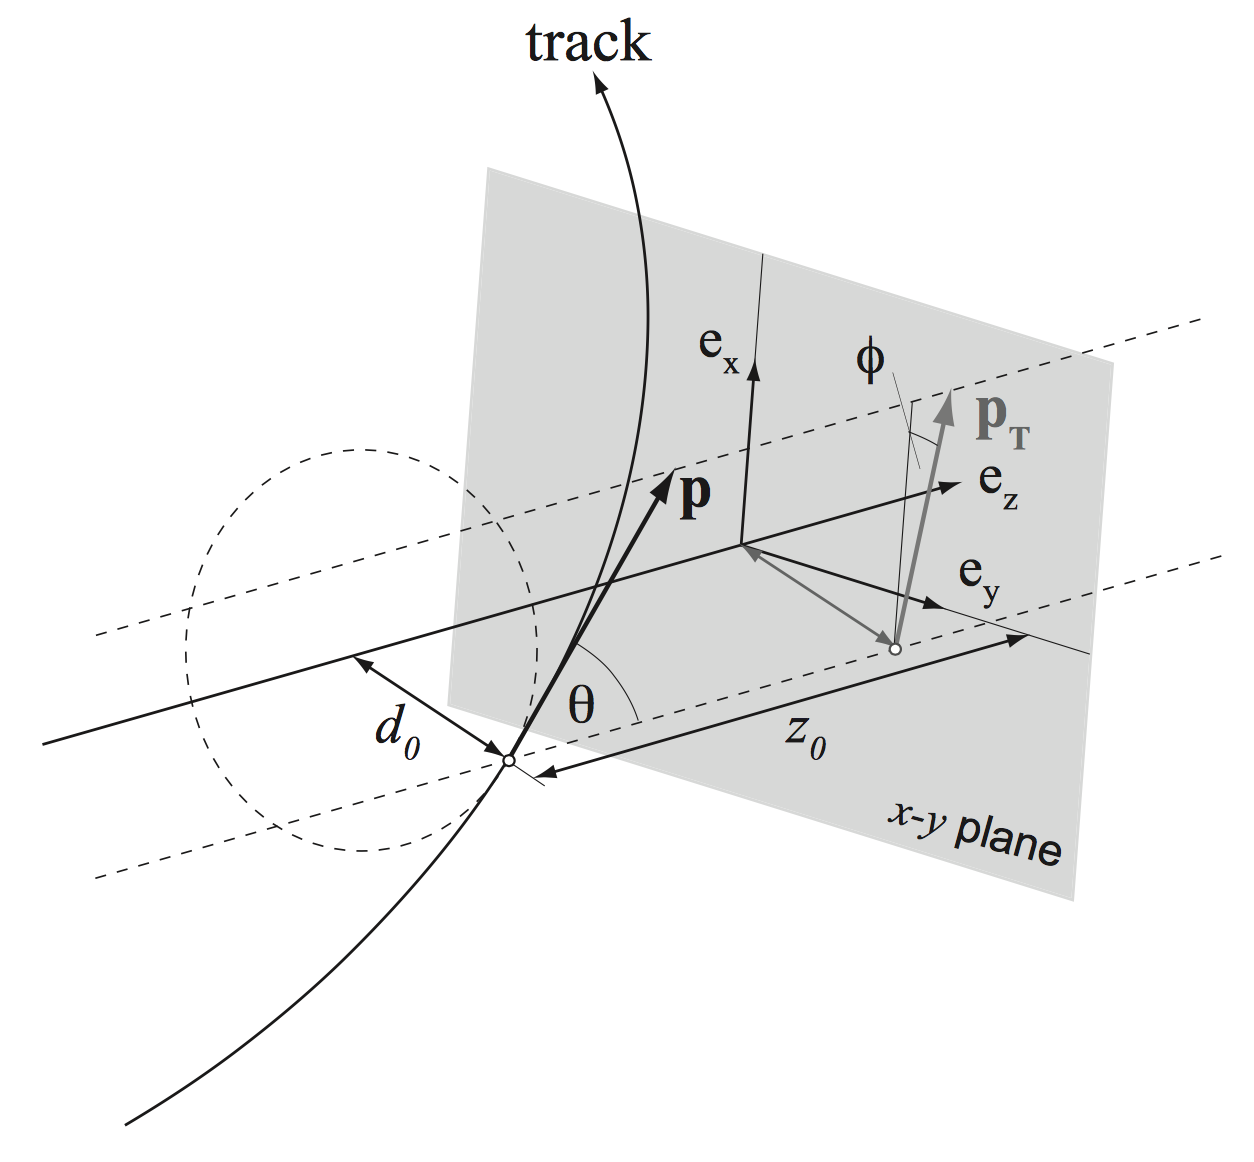
\includegraphics[width=0.6\textwidth]{Images/tracking_det/ImpactParameters.png}
\caption{Scheme of the track helix). The tracks is defined in the perigee representation at the point of closest approach P and the referee position R}
\label{pic:impact_param}
\end{figure}

A set of five helix parameters ($d_0$,$z_0$,$\phi$,$cot(\theta)$,$\frac{Q}{p_T}$) can describe a track in the solenoidal magnetic field B, as shown in Figure \ref{pic:impact_param}.
In particular the first two parameters are referred as transverse impact parameter ($d_0$) and longitudinal impact parameter ($z_0$).
The first one ($d_0$) is defined as the distance of closest approach to the beam-line, while the second one ($z_0$) as the value of z of the point on the track that determines $d_0$.
Because the errors on the five track parameters are not independent, they are described by a $5\times5$ covariance matrix C.
%The diagonal elements are the squared sigma values C = cov( p ) = σ 2 . The off-diagonal terms are C = cov( p , p ) = ρ σ σ , with ρab the aa aa ab ababab correlation between parameter pa and parameter pb (|ρab| ≤ 1). If pa and pb are independent ρab = 0. If pa and pb are linearly related |ρab| = 1. 
Because in a very good approximation the variables in the (x, y) plane and the (r, z) plane are independent, only $2\times4$ covariances are not zero: $cov(Q/p , \phi )$, $cov(Q/p , d_0)$, $cov(\phi , d_0)$ and $cov(cot(\theta), z_0)$. Covariance matrices always symmetric, invertible and positive definite.
The errors of the impact parameters are derived from the covariance matrix and they depends on the geometrical characteristics of the detector and on the multiple scattering.
A simple example to evaluate the basic tracking performance is based on equally spaced detector.
For the plane containing the magnetic field, a detector made by $N+1$ layers, each one having a measurement error $\sigma$, has an error on the impact parameter ($z_0$) measurement given by:
\begin{equation}
\sigma_{z_0}^2 = \sigma_a^2 +\sigma_b^2 Z_c^2 = \frac{\sigma^2}{N+1} +\frac{\sigma^2}{N+1} \frac{12N}{N+2}\frac{Z_c^2}{L^2}
\end{equation}
where the formula is calculated choosing a reference frame with the origin at the center of the track, and $L=Z_N-Z_0$, $Z_c = (Z_N+Z_0)/2$ and the error on track parameters ($\sigma_a$ and $\sigma_b$) are not correlated.
The above formula shows how the error of the impact parameter ($z_0$) depends on the error of the slope of the track ($\sigma_b$) and on the distance of the center of the spectrometer from the interaction point ($Z_c$).
The impact parameter resolution is also affected by multiple scattering so that a more precise calculation is given by:
\begin{equation}
\sigma_{z_0} =\sqrt{ \frac{\sigma^2}{N+1} +\frac{\sigma^2}{N+1} \frac{12N}{N+2}\frac{Z_c^2}{L^2}} \oplus \frac{k}{p_T} 
\end{equation}
where k is derived from \ref{eq:mult_scat}.
The calculation of the transverse impact parameter is similar but it contains additional terms that depends on the magnetic field; to minimize the error on the impact parameter the following characteristics are required:
\begin{itemize}
\item excellent spatial resolution $\sigma$ is needed;
\item make the spectrometer as long as possible to reduce the error on the slope;
\item place the spectrometer as close as possible to the interaction point.
\item the impact of multiple scattering is important at low energy
\end{itemize}

%The uncertainty on the transverse impact parameter can be derived with a simplified model involving only 2 layers:
%\begin{equation}
%\sigma_{d_0}=\frac{r_2 \sigma_1 \oplus r_1 \sigma_2}{(r_2 - r_1)} \oplus \frac{k_1 r_1}{p_T}
%\end{equation}
%where the second term $\frac{k_1 r_1}{p_T}$ comes from contribution of multiple scattering.

%The simplified model gives some hints about the geometry of a tracking detector for a good impact parameter resolution.
%\begin{itemize}
%\item the innermost radius should be as close as possible to the interaction point
%\item the outermost radius should be far from the interaction point
%\end{itemize}

\subsubsection{Momentum resolution}
Momentum resolution could be explained studying the case of the plane transverse to the magnetic field, considering a spectrometer placed at the position $X_0,...,X_N$. The spectrometer length is $L = X_N - X_0$. The error on the coefficient of the quadratic term is:
\begin{equation}
\sigma_c^2 = \frac{\sigma^2}{L^4}A_N,\quad A_N=\frac{720N^3}{(N-1)(N+1)(N+2)(N+3)}
\end{equation}
Since $c=-R^{-1}$ the error on the transverse momentum pt is given by:
\begin{equation}
\frac{\delta p_t}{p_t} = \frac{p_t}{q}\frac{\sigma}{BL^2}\sqrt{A_N}=p\frac{\sigma}{0.3BL^2}\sqrt{A_L}
\end{equation}
in units of GeV, Tesla and metres. The formula illustrates the basic features of the momentum measurement with a magnetic spectrometer:
\begin{itemize}
\item the relative transverse momentum resolution is proportional to the transverse momentum;
\item the strong dependence on the spectrometer length L calls for large detectors to achieve good momentum resolution;
\item the transverse momentum resolution is inversely proportional to the magnetic field;
\item the dependence on the number of measured coordinates is weak; however the number of coordinates is important for the robustness of the pattern recognition.
\end{itemize}
%2.3. Multiple scattering
%The uncertainty of the track parameters is affected by multiple scattering of the charged particle by the material of the spectrometer. A particle of momentum p and unit charge traversing a path length x of material, characterized by a radiation length X0, is deflected by multiple Coulomb scattering from nuclei. The projection of this deflection angle on any plane containing the original direction is roughly Gaussian distributed around zero with a root mean square width given by \ref{eq:mult_scat}.
%Excellent spatial resolution is obtained with silicon detectors designed to have $\sigma\simeq10 \mu m$ or better. As such detectors are very expensive, the maximum spectrometer length L is limited. To overcome this limitation, the spectrometers are usually split into an inner vertex detector and a central tracking detector. The latter can be made long (large L) making the error on the slope small. Compact pixel vertex detectors provide excellent spatial resolution very near to the interaction point.
%The random deflection smears the position measurements and introduces a correlation among position measurements downstream of the material causing the deflection. Assuming that the position accuracy is dominated by multiple scattering, the momentum resolution for a spectrometer of length L and N + 1 equally spaced position measurements is given by [8, 9] 􏱠
%δpt = 1 0.0136 CN , where CN is an N-dependent coefficient [9] which is equal to 1.3 within 10% accuracy. When multiple scattering dominates, the relative momentum resolution does not depend on the momentum and has a weak dependence on the length of the spectrometer.
%At colliders, secondary vertices of short lived particles are contained within the beam pipe. For particles of low momentum the multiple scattering in the material of the beam pipe becomes a significant source of error. A track measured with infinite precision outside the beam pipe when extrapolated to the origin misses the primary vertex by a randomly distributed distance d which has roughly Gaussian distribution with a width drms = Rbpθbp, where Rbp is the radius of the beam pipe and θbp the rms multiple scattering angle due to the beam pipe material.
%\subsubsection{Vertices algorithms}
%\subsubsection{B-tagging algorithms}

\subsubsection{Mathematical determination for the vertex position}
\label{sec:kalman_filter}
The determination of the vertex position is a well defined task: it consists in taking N input tracks and in determining their intersection, which results in the estimation of the vertex position and its related error. There are several methods that could be used for this task.
The easiest way to estimate the vertex position and its related error is to minimize the $\chi^2$, but in general this approach is rather slow due to the size of the covariance matrix to be growing with the number of tracks.
A significantly faster method is the application of the Kalman filter, firstly applied in vertex fitting in~\ref{Giac_62}.
%A Kalman filter is usually applied to linear dynamic systems, which at every step k are described by a state vector $\vv{r}$. The evolution of the state vector from step $k-1$ to step k is described by the linear transformation:
%\begin{equation}
%\vv{r}_k = F_{k-1}\cdot \vv{r}_{k-1} + \vv{w}_{k-1}
%\end{equation}
%where $F_{k-1}$ is the propagation matrix and $\vv{w}_{k-1}$ is a random noise contribution to the system during the propagation step. At every step a new measurement constrains the system, where the measurements $\vv{m}_k$ needs to be described as a linear function of the state vector $\vv{x}_k$ with associated Gaussian noise $\vv{\epsilon}_k$.
%Given such a linear dynamic system, the Kalman filter provides:
%\begin{itemize}
%\item Filtering: the optimal recursive estimator of the present state vector $\vv{x}$ given all previous measurements
%\item Prediction: the optimal estimation of the state vector at a future time, given all past measurements.
%\item Smoothing: an improved estimation of the state vector at some time in the past, given all measurements up to the present time.
%\end{itemize}
In the case of vertexing the application of a Kalman filter the single, $k$ is interpreted as the addition of a track to the vertex. The state vector is given by the vertex position and the track momentum corresponding to the track added at step k: $\vv{x}_k = (\vv{r}, \vv{p}_k)$.
After a track being iteratively included in the fit, the Kalman filter provides the estimation of the vertex and related covariance matrix corresponding to the minimization of the vertex $\chi^2$, including all the tracks considered up to that point. After all the tracks are added to the fit, the problem of estimating the vertex position is solved.
The same does not hold for track momenta evaluated at estimated vertex position, which should not provide an improved estimate of the track momenta giving by constraining the track to pass through the vertex; since the momenta are updated on at certain step k, they do not take in account all changes in the vertex position taking place at all steps after k.
In order to get  complete estimate of them, the final result needs to be propagate to earlier Kalman filter update steps, which is usually done at the smoothing step. The smoothing procedure is also needed to get the correct estimation for the $\chi^2$ contribution given by a single track k, which needs again to rely on the final estimate of the vertex position.
In case of vertex fit the evolution equation becomes trivial:
\begin{equation}
\vv{x}_k = \vv{x}_{k-1}
\end{equation}
since no propagation and no noise addition needs to be performed, while the measurement equation gives the linear relation between the track measurements and the vertex position and track momentum;
\begin{equation}
\vv{m}_k = \vv{c}_0 + A\vv{r} + B\vv{p}_k
\end{equation}
Since the Kalman filter is an iterative procedure, the components of the state vector need to be initialized; when the initial estimate is very poor is sufficient to inflate the error matrix in order to make the influence of the starting vector negligible in the fit.
\pagebreak
